% ReScience C article content. Every simulated number is a macro from
% ../../paper/results.tex, written by scripts/make_figures.py from data/.

\section*{Introduction}
Enderling et al.\ \cite{enderling2009} introduced a cellular automaton of cancer stem cells,
which divide without limit, and their non-stem progeny, which can divide only a limited
number of times. Their central and counter-intuitive result is that increasing the
spontaneous death rate of non-stem cells can make tumours grow larger in the long run:
dying non-stem cells free space in which stem cells can divide, so the stem cell pool, and
eventually the tumour, expands. Poleszczuk and Enderling \cite{poleszczuk2014} later gave a
compact specification of the model with explicit parameter values and a reference tumour
size. We re-implemented the model from this specification and compared it with both papers.
The authors' code, announced in \cite{poleszczuk2014}, could not be found.

\section*{Methods}
\paragraph{Model.} As specified in \cite{poleszczuk2014}: a two-dimensional square lattice
with one cell per \SI{10}{\micro\meter} site and Moore neighbourhood. Stem cells are immortal
and divide without limit; at division they produce another stem cell with probability
$p_s=0.1$, otherwise a non-stem cell with proliferation capacity $\rho_{\max}=10$. A non-stem
cell divides at most $\rho_{\max}$ times; its capacity decreases at each division and is
inherited by the daughter. A cell needs a free neighbouring site to divide or move; cells
without one are quiescent. At each hourly step, the cells present at the start of the step
are updated once, in random order: with probability $p_d=1/24$ (cell cycle 24~h) a cell
attempts to divide, otherwise it migrates with probability $p_m$ to a free neighbour chosen
uniformly. One stem cell starts in the centre; tumours grow for 180 days.

\paragraph{Spontaneous death.} A non-stem cell dies with probability $\alpha$ at a division
attempt, or when its capacity is exhausted. \cite{poleszczuk2014} does not say when death is
tested; we took this rule from the later methods chapter of the same group
\cite{poleszczuk2016}.

\paragraph{Migration.} \cite{poleszczuk2014} gives the motility as $\mu = \SI{100}{\micro\meter}$
per day and $p_m = \mu\,\Delta t$. Read in cell widths (10 cells per day, 24 steps per day),
$p_m = 10/24$; read literally in micrometres, $p_m$ exceeds one, i.e.\ a cell that does not
divide always attempts to move ($p_m=1$). We report both readings.

\paragraph{Implementation and ensembles.} C++ with one tumour per OpenMP thread, fixed
lattices of $1000\times1000$ sites ($1400\times1400$ for the migration sweep, whose largest
tumours are bigger) that no tumour reached the edge of, and the 64-bit Mersenne Twister of the
C++ standard library seeded per tumour. \CATumours{} tumours per
death rate ($\alpha$ = 0, 0.01, 0.05, 0.1, 0.2 and 0.3) with $p_m=10/24$; 16 tumours per
migration probability. Means are given with standard errors.

\section*{Results}
\paragraph{The paradox is reproduced.} Tumours grow larger as the death rate of non-stem cells
increases from 0 to 0.2: \CAParadoxLow{} cells at $\alpha=0$ against \CAParadoxHigh{} at
$\alpha=0.2$ after 180 days, with \CAStemRatio{}-fold more stem cells (Table~\ref{tab:paradox},
Figure~\ref{fig:paradox}), as reported in \cite{enderling2009}. More than 70\,\% of cells have
no free neighbour (\CAQuiescent{} at $\alpha=0.01$), as reported in \cite{poleszczuk2014}.

\begin{table}[htbp]
\centering\small
\caption{Tumours after 180 days ($p_m=10/24$, \CATumours{} tumours each; mean $\pm$ standard
error).}
\label{tab:paradox}
\begin{tabular}{rrrr}
\toprule
$\alpha$ & cells & stem cells & without free neighbour \\
\midrule
0 & 56{,}922 $\pm$ 3{,}068 & 150 $\pm$ 9 & 70.2\,\% \\
0.01 & 60{,}692 $\pm$ 2{,}604 & 173 $\pm$ 7 & 71.3\,\% \\
0.05 & 85{,}645 $\pm$ 3{,}529 & 305 $\pm$ 13 & 75.6\,\% \\
0.1 & 116{,}699 $\pm$ 3{,}967 & 571 $\pm$ 19 & 78.1\,\% \\
0.2 & 167{,}773 $\pm$ 4{,}932 & 1811 $\pm$ 53 & 83.1\,\% \\
0.3 & 179{,}227 $\pm$ 4{,}500 & 4794 $\pm$ 122 & 84.7\,\% \\
\bottomrule
\end{tabular}

\end{table}

\begin{figure}[htbp]
\centering
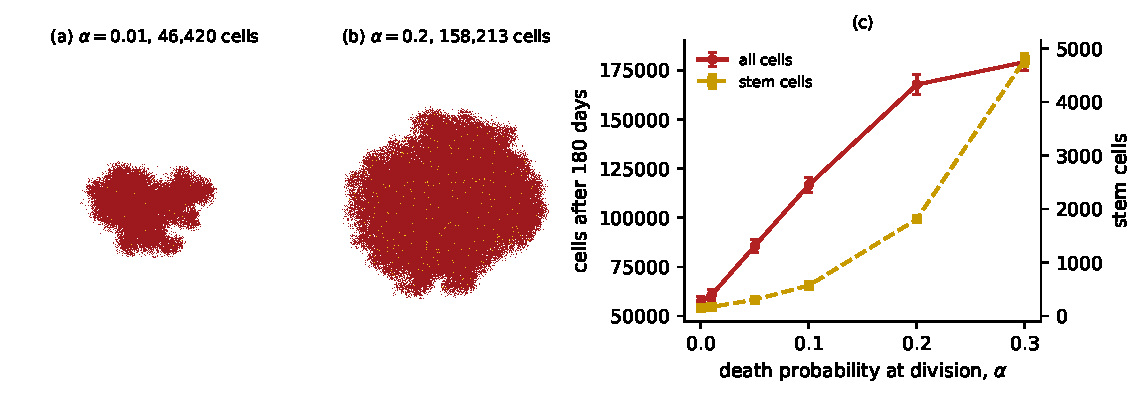
\includegraphics[width=\linewidth]{../../figures/ca_paradox.pdf}
\caption{Tumours after 180 days. (a, b) One tumour at $\alpha=0.01$ and $\alpha=0.2$ (same
seed; stem cells in yellow; each panel \SI{7}{\milli\meter} wide). (c) Final numbers of cells and
stem cells against $\alpha$ (mean $\pm$ s.e., \CATumours{} tumours each).}
\label{fig:paradox}
\end{figure}

\paragraph{The published tumour size is not reproduced.} \cite{poleszczuk2014} reports about
140{,}000 cells after 180 days at $\alpha=0.01$. With $p_m=10/24$ we obtain \CASizeCellWidths{}
cells (mean of \CATumours{} tumours), with $p_m=1$ \CASizeLiteral{} (16 tumours). The final size
grows steeply with $p_m$, and the published size corresponds to $p_m\approx\CAPmMatch{}$ in our
implementation (Figure~\ref{fig:migration}).

\begin{figure}[htbp]
\centering
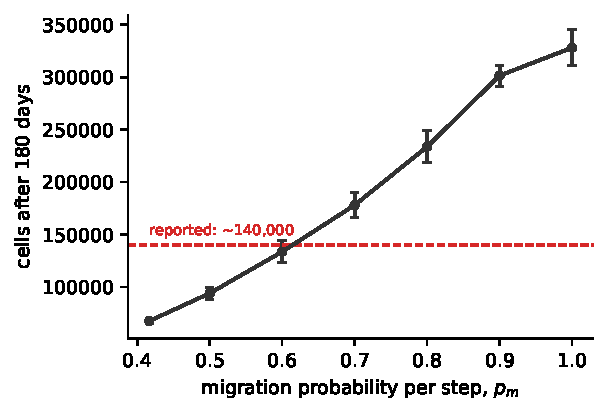
\includegraphics[width=0.6\linewidth]{../../figures/ca_migration.pdf}
\caption{Tumour size after 180 days against the migration probability per step
($\alpha=0.01$, 16 tumours each, mean $\pm$ s.e.). Dashed: about 140{,}000 cells reported in
\cite{poleszczuk2014}. The two readings of $\mu=\SI{100}{\micro\meter}$ per day are $p_m=10/24$
and $p_m=1$.}
\label{fig:migration}
\end{figure}

\section*{Discussion}
The qualitative result of \cite{enderling2009}, the paradoxical growth of tumours with a higher
non-stem cell death rate, is robust: it follows from an independent implementation of the
published specification. The quantitative tumour size is not reproduced, because the
specification leaves open two rules that strongly affect it: the migration probability per
step and the moment at which spontaneous death is tested. Between the two readings of the
motility, the final size changes more than five-fold. Quantitative uses of this model should
state these rules explicitly; ours are given above and in the code. We contacted the
corresponding author about the migration rule and the original code.

\section*{Code, data and reproducibility}
Code: \url{https://github.com/quantumproteinsai/rescience-bozic2013-enderling2009}, archived at
\href{https://doi.org/10.5281/zenodo.23437598}{doi:10.5281/zenodo.23437598}. The model is
\texttt{src/ca/ca\_reference.cpp}; \texttt{make all} rebuilds it and regenerates every number,
table and figure from fixed seeds. For reviewers, \texttt{make quick-check} reproduces 11 representative published results exactly, from scratch, in about two minutes on a laptop. The exact numbers are reproduced with GCC and its standard
library; other C++ standard libraries implement the random distributions differently and give
statistically equivalent, not identical, results.

\section*{Use of AI assistance}
The software, simulations, analyses and the first draft of this article were produced with an
AI coding assistant (Claude Opus 5.5, Anthropic, used through Claude Code), under the direction
of the author, who defined the study, chose the comparisons, checked the results against the
original publications and revised the text. The AI is not an author; the author takes full
responsibility for the content.

\section*{Funding}
This work received no specific funding.
